\chapter{Implementation}
% (more or less telling whats in my code; implementation details; describing dataset; which network and which hyper parameters do I use; how does the application look like)
\section{Setup}

In order to conduct the training process described by the methods used in the previous chapter, it is necessary to have a computer with a powerful GPU in order to speed up training. For this Master thesis, the experiments/training was conducted on a Nvidia Titan X (Pascal) GPU with 12 GB of memory. 
\newline\newline
The framework used for Machine Learning is TensorFlow. It provides a specific software package for GPU usage which is called 'tensorflow-gpu' and was installed in version '1.14.0'. Furthermore, Keras is used on top of Tensorflow, which is a neural network library that makes faster and easier to interact with the underlying Machine Learning framework. Keras is used in version 2.3.1.
\newline\newline
Further important third-party software packages include:
\begin{itemize}
    \item Keras-VggFace: Version 0.6
    \item MTCNN:         Version 0.1.0
    \item OpenCV:        Version 4.1
\end{itemize}
All these frameworks and packages are being used inside the Python programming language. The utilized version is 3.6.


\section{Dataset}
\textbf{Background}
\newline
The selected AFEW-VA dataset \citet{Kossaifi:2017:AFEW-VADatabase} is based upon the Acted Facial Expressions In-The-Wild database (AFEW) proposed in \citeyear{Dhall:2012:AFEW} by \citet{Dhall:2012:AFEW}. The AFEW dataset is composed of video clips that try to depict a real-world environment. It is capturing facial expressions, natural head pose movements, occlusions, subjects' races, gender, diverse ages, and multiple subjects in a scene. The authors labeled the video clips with one of six basic expressions: anger, disgust, fear, happiness, sadness, surprise, or neutral.
\newline\newline
The AFEW-VA dataset\citep{Kossaifi:2017:AFEW-VADatabase} uses the same underlying real-world video data, but is not annotating their clips with one of six basic expressions. Instead it is using the two dimensional affective space with valence and arousal. While valence expresses how positive or negative an emotion is, arousal expresses how strong or weak an emotion is.
\newline\newline
Furthermore, as the name of the dataset already suggests, the dataset is comprised of data that was collected under 'In-The-Wild' conditions. Hereby, 'In-The-Wild' refers to real-life conditions in video clips, which make it very difficult to recognize emotions. \citet{Salah:2018:VideoBasedER} explains that these difficulties can be caused by, for example, uncontrolled illumination or uncontrolled video quality due to a different recording medium, like webcams by individuals vs. professional cameras. Such 'In-The-Wild' data is usually acquired from talk shows, movies or other naturalistic interactions. 
\newline\newline
As the research conducted during this Master thesis is intended to serve as a basis for a further real-life application in video-call scenarios, it was clear that the dataset needs to be as close to 'In-The-Wild' conditions as possible. Furthermore, it was decided that it is more important to capture as much of an emotions information as possible rather than placing value on the interpretation of emotions. As a result, the AFEW-VA dataset got chosen because of its 'In-the-Wild' conditions, its 2D Affective Space model for emotion representation and its backing by the scientific community by providing comparable results.
\textbf{Data structure}
\newline
The dataset is split into 600 folders, each standing for a different video clip. Each video clip is taken from a different subject. Each of these folders holds multiple frames which together make up the video clip. Moreover, the folder also holds a .json file which holds the label for each frame and describes it in terms of valence, arousal and landmark points.
\newline\newline
This .json file contains for each frame a value for the valence and another value for the arousal. Both values have an annotation level ranging from -10 to +10 in full integer values. This results in a total of 21 levels.\citep{Kossaifi:2017:AFEW-VADatabase} Additionally, the file also includes pre-labeled landmarks for face detection purposes. These landmarks are as of now (30th of September 2020) not utilized, as different pre-trained third-party modules are being used for the task of face detection and landmark determination.
\newline\newline
\textbf{Benchmark}
\newline
In order to objectively compare the results from the original AFEW-VA paper proposed by \citet{Kossaifi:2017:AFEW-VADatabase}, it is essential to lay out the circumstances under which the results were obtained. In the case of the AFEW-VA paper\citep{Kossaifi:2017:AFEW-VADatabase}, as well as the Simulatenous VA prediction paper \citep{Handrich:2020:SimultaneousPredVA}, the data got divided in 5 disjoint folds in a subject-independent manner, meaning a subject does not appear in different folds. Subsequently, they performed a 5-fold-cross-validation for the prediction of valence and arousal values for each frame of a video clip.\citep{Kossaifi:2017:AFEW-VADatabase}
\newline\newline
\citet{Roehrich:2020:TrainValidateTest} argues that when comparing different models it is not enough to use a training and a testing set, as it might still be possible that one model is better than the other due to randomness during the training process. Thus, additionally to the above mentioned approach of creating 5 folds in a subject independent manner, it is important to separate the folds into training, validation and testing subsets. The split of the database into subsets is shown in figure \ref{fig:TrainTestSplit} and these subsets fulfill the following purposes:

\begin{itemize}
    \item The training dataset will be used for the actual training of the model
    \item The validation dataset is used for testing during the training process. Thus, it serves as a metric that needs to be improved by, for example, adapting the model architecture. Moreover, it serves as the metric for the EarlyStopping meachanism which ends the training process when the observed metric stales in its performance
    \item The testing dataset is all about the actual measurement of the model's performance on a third previously unseen dataset
\end{itemize}

\begin{figure}[H]
  \begin{center}
  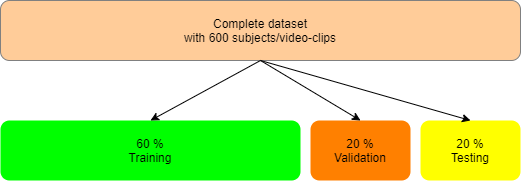
\includegraphics[angle=0, width=0.6\textwidth]{Figures/TrainTest_Split.png}
  \caption{Train, Validation and Test split}
  \label{fig:TrainTestSplit}
  \end{center}
\end{figure}

For the final results of the proposed approach, 5-fold-cross-validation was conducted by splitting the 600 subjects/video-clips into 5 folds with each containing 120 subjects. 4 out of those 5 folds were used for training, while 1 fold was reserved for the evaluation of the model after the finished training. The 4 folds were again split into training and validation, with 1 fold serving as the validation set. This approach can also be seen in figure \ref{fig:CrossValidationSplit}.

\begin{figure}[H]
  \begin{center}
  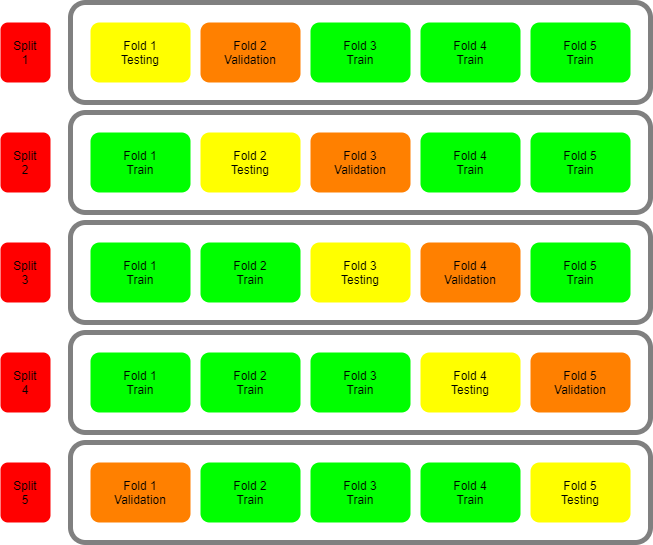
\includegraphics[angle=0, width=0.8\textwidth]{Figures/CrossValidation_Split.png}
  \caption{Cross-Validation split}
  \label{fig:CrossValidationSplit}
  \end{center}
\end{figure}

This approach ensures that there is no overlap, in terms of subjects, between the training and testing/evaluation. Therefore, the subset for the evaluation of the model performance contains only frames from subjects that were previously not seen by the model during the training process.



% \begin{quote}
%     To compare the performance of various features, we sampled regularly an equal number of frames from each sequence to obtain a set of frames representative of the whole dataset, which we then divided in 5 disjoint folds in a subject-independent manner (i.e. a subject does not appear in two different folds). We then performed a 5-fold cross-validation (i.e. we iteratively used one of the set for testing and the other 4 for training) to predict the valence and arousal values for each frame. \citep{Kossaifi:2017:AFEW-VADatabase}
% \end{quote}

\section{Architecture}

\begin{figure}[H]
  \begin{center}
  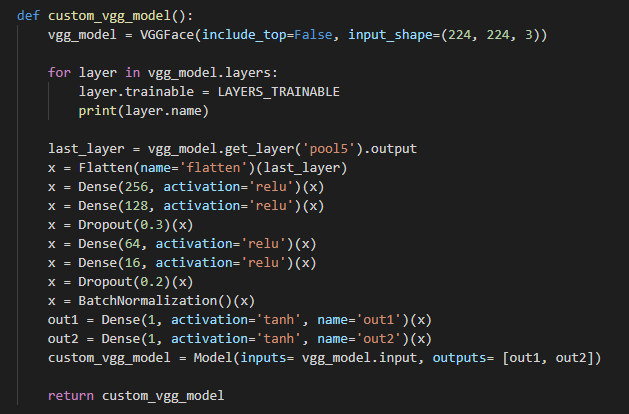
\includegraphics[angle=0, width=1.0\textwidth]{Figures/model_architecture.PNG}
  \caption{Neural Network Architecture}
  \label{fig:NNArchitecture}
  \end{center}
\end{figure}

In figure \ref{fig:NNArchitecture} the architecture of the neural network is being described. Firstly, in line \#2, the pre-trained VGGFace model is being loaded with 'resnet50' as its neural network architecture. This means it will return a resnet50 architecture that was pre-trained on the VGGFace2 dataset. Furthermore, the parameter 'include\_top' is set to False. It is necessary to leave out the last layers that were pre-trained on face detection and replace them through custom layers that can learn the emotions from a person's face. Moreover, the input shape is being defined for the images that the model expects and the pooling method used for reducing the output to a vector is defined with 'avg'.
\newline\newline
From line \#5 to line \#10 the pre-trained layers of the VGGFace model are either set to trainable or non-trainable. This mechanism is used for the fine-tuning strategy as part of the training process. Namely, during the first 3 epochs only the weights of the custom layers are updated (=trained) and the layers of the VGGFace model are frozen (=set to non-trainable). Afterwards all layers are set to trainable and weight changes take place in all layers of the here described architecture.
\newline\newline
The output layer of the VGGFace model is being accessed in line \#12 and gets flattened by one dimension in line \#13 in order to fit the dimension requirements for the following layers. 
\newline\newline
The next four lines from line \#15 to line \#18 comprise the block of fully-connected layers. As it can be seen in line \#16 there is only one Dense layer with 1024 units and a rectified linear unit (relu) as an activation function. Around this Dense layer two Dropout layers are being found which randomly discard information inside the neural network. Together with the Batch Normalization layer, the Dropout layers act as a regularizer during the training process. Thus, they make it more difficult for the model to learn, while making it more robust and generalize better, which means that it perform better on previously unseen data.
\newline\newline
The choice of only using a single Dense layer in the block of fully connected layers is based upon a paper \citep{Pittaras:2017:FineTuningStrategiesComparison} that compared different fine tuning strategies on pre-trained neural networks. \citet{Pittaras:2017:FineTuningStrategiesComparison} found out during their experiments that

\begin{quote}
    increasing the depth of a pre-trained network with one more fully-connected layer and fine-tuning the rest of the layers on the target dataset can improve the network’s concept detection accuracy compared to other fine-tuning approaches. \citep{Pittaras:2017:FineTuningStrategiesComparison}
\end{quote}

After an image has passed through the layers of the VGGFace model and the four custom defined fully connected layers, the result gets fed into the output layer. In this case, the output is split up into two variables, each separately defined by a Dense layer with a 'tanh' activation. The 'tanh' activation makes sure that the output gets resized to any floating-point number in the range of -1 to +1.
\newline
This split can be seen in the line \#20 and \#21 and is done in order to apply the evaluation metric to each output individually, which makes it possible to neatly visualize the outcomes.
\newline\newline
Next in the code, the layers in the pre-trained VGGFace model are set to non-trainable during the first three epochs of the training process. Afterwards the variable 'is\_trainable' gets switched to True and all the layers are set trainable. This signifies, that the weights in the neurons are being updated during the training process.

%%%%%%%%%%%%%%%%%%%%%%%%%%%%%%%%%%%%%%%%%%%%%%%%%%%%%%%%%


\section{Fine-tuning}
\subsubsection{ResNet50 model}
ResNet50, short for Residual Network, is a very deep neural network architecture that was invented for the purpose of image classification, resulting in winning the ImageNet challenge in 2015. \citep{Dwivedi:2019:ResNetInKeras}

\begin{figure}[H]
  \begin{center}
  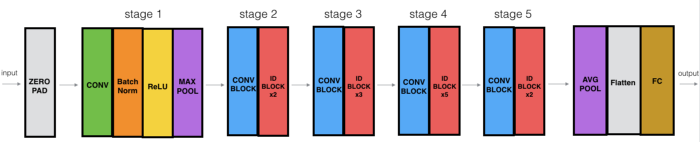
\includegraphics[angle=0, width=1.0\textwidth]{Figures/resnet50.png}
  \caption{ResNet50 Architecture \citep{Dwivedi:2019:ResNetInKeras}}
  \label{fig:ResNet50Architecture}
  \end{center}
\end{figure}

\begin{quote}
    The ResNet-50 model consists of 5 stages each with a convolution and Identity block. Each convolution block has 3 convolution layers and each identity block also has 3 convolution layers. The ResNet-50 has over 23 million trainable parameters. \citep{Dwivedi:2019:ResNetInKeras}
\end{quote}

This architecture of the ResNet50 model exhibits a very deep-layered neural network. However, the biggest challenge with deep-layered neural networks is their difficulty to train them because of the notorious vanishing gradient problem. This may result in rapid saturation and degradation of performance. In order to fight this problem, ResNet introduced a novel concept, named skip connection. The approach adds together the result of the convolutional block with its original input and outputs the result of this operation. \citep{Dwivedi:2019:ResNetInKeras}\newline
This concept is also illustrated in the following figure \ref{fig:ResNet50SkipConnection}:

\begin{figure}[H]
  \begin{center}
  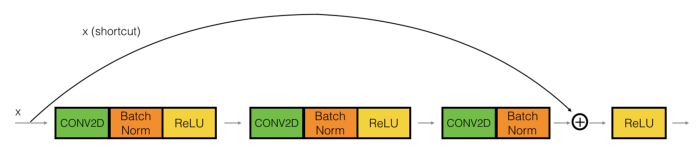
\includegraphics[angle=0, width=0.9\textwidth]{Figures/skip_connection.png}
  \caption{ResNet50 Skip Connection\citep{Dwivedi:2019:ResNetInKeras}}
  \label{fig:ResNet50SkipConnection}
  \end{center}
\end{figure}

\citet{Dwivedi:2019:ResNetInKeras} argues that this approach is helpful in mitigating the problem of vanishing gradients, as its skip connection concepts firstly, provides an alternate short cut path for gradients to flow through and sencondly, ensures that the subsequent layer will perform at least as good as the previous layer.

\subsubsection{Pre-trained network}
As recommended by \citet{Chollet:2017:DeepLearningPython} using a pre-trained neural network is a highly effective approach to deep learning on a small image dataset. The AFEW-VA dataset with its 600 video clips, resulting in about 30.000 frames to train on can be considered a rather small dataset.\citep{Kossaifi:2017:AFEW-VADatabase}

\begin{quote}
    A pretrained network is a saved network that was previously trained on a large dataset, typically on a large-scale image-classification task. If this original dataset is large enough and general enough, then the spatial hierarchy of features learned by the pretrained network can effectively act as a generic model of the visual world, and hence its features can prove useful for many different Computer Vision problems, even though these new problems may involve completely different classes than those of the original task. \citep{Chollet:2017:DeepLearningPython}
\end{quote}

\citet{Chollet:2017:DeepLearningPython} further elaborates that using a pre-trained network for small-data problems makes deep learning a very effective approach due to its portability of learned features across different problems.
\newline\newline
This is why, it seemed promising to solve the Emotion Recognition challenge at hand with a neural network, that was pre-trained on a more general and holistic dataset. Therefore, it was chosen to use a ResNet50 neural network architecture pre-trained on a large-scale face recognition dataset containing 3.31 million images, called VGGFace2 \citep{Cao:2018:VGGFace2}.


\subsubsection{Fine-tuning strategy}
The layers inside a deep neural network are commonly divided into the convolutional base and the classifier. In the proposed approach, the ResNet50 architecture serves as the convolutional base, while the classifier is being added by manually defining the respective layers. Therefore, the convolutional base is initialized with its pre-trained weights, while the classifier isn't yet trained.
\newline\newline
The exact steps for fine-tuning a neural network are summarized by \citet{Chollet:2017:DeepLearningPython} as follows:
\begin{enumerate}
    \item Add your custom network on top of an already-trained base network
    \item Freeze the base network
    \item Train the part you added
    \item Unfreeze some layers in the base network
    \item Jointly train both these layers and the part you added
\end{enumerate}

\citet{Chollet:2017:DeepLearningPython} further highlights, that if the classifier isn't already trained and the whole model, including the pre-trained convolutional base, gets fine-tuned, then the error being propagated through the network will be too big. This might result in the destruction of previously learned representations by the layers. As a result, the custom network part (in the case of the here proposed approach: the classifier) needs to be trained first separately as mentioned in step 3. 
\newline\newline
As mentioned in step 4 only some layers of the base network are being unfrozen and thus, used during training. According to \citet{Chollet:2017:DeepLearningPython} it is more useful to fine-tune the higher layers because these encode more specialized features and need to be readjusted to the new problem. Fine-tuning all the layers is theoretically possible, although it would increase the risk of overfitting. Therefore, it is better to keep lower layers of the convolutional base frozen as they encode more generic features which can be useful for a wide variety of tasks/problems.


% \citet{Yan:2016:MultiClueFusion} made use of multi clue fusion to further enhance the accuracy of an emotion recognition in the Wild. They showed that with using only the VGGFace model as a predictor for the Emotion Recognition challenge, they got a surprisingly high accuracy of about 36 per cent. They also mention that it the model will perform better as they recognize emotions over multiple frames and conduct fine-tuning on the VGGFace model. (Fintuning = the adaption of a pre-trained model to the current challenge, usually done together with a new dataset)
% \newline\newline
% Furthermore, they detect faces with Single Shot Detector (SSD) and whenever it fails, they crop the image manually so far, that the detector "has" to detect it. However, in the approach describe in this thesis, images with a non-detectable face will be passed into the model in their original size. Thus, no manual cropping is being conducted. Additionally, they focus on the concept of action units (AU) together with landmarks. They define a facial expression is a combination of several action units (AU) movements, with the action units being the trajectories of vital facial
% landmarks.
% \citep{Yan:2016:MultiClueFusion}

%%%%%%%%%%%%%%%%%%%%%%%%%%%%%%%%%%%%%%%%%%%%%%%%%%%%%%%%%

\section{Metrics}
Metrics in Machine Learning are used to evaluate the performance of a Neural Network. Probably the most widely used metric is 'accuracy' which tells you about the share of correctly predicted data points. 
\newline\newline
As the present challenge of predicting values for valence and arousal is better solved through regression, the 'accuracy' metric will not be able to deliver meaningful and actionable results. Instead it is better to use better suited metrics, as were already proposed in previous paper. The author decided on using the RMSE (Root-mean-squared error) and CORR (Pearson product-moment correlation coefficient) as metrics for this challenges.
\newline\newline
RMSE gives the observer a notion of how close the predicted values are to the actual values. It can also be defined as follows:

\begin{quote}
    Root Mean Square Error (RMSE) is the standard deviation of the residuals (prediction errors). Residuals are a measure of how far from the regression line data points are ... In other words, it tells you how concentrated the data is around the line of best fit. \citep{2020:RMSE}
\end{quote}

The CORR metric tells you how strong the relationship between the prediction and the actual label is. In other words:

\begin{quote}
    CORR gives information about the magnitude of the association, or correlation, as well as the direction of the relationship. \citep{2020:PearsonCorrelation}
\end{quote}

The RMSE metric is additionally used as the to-be-optimized loss function during the training process. Both metrics are being custom implemented by the following source code:

\begin{figure}[H]
  \begin{center}
  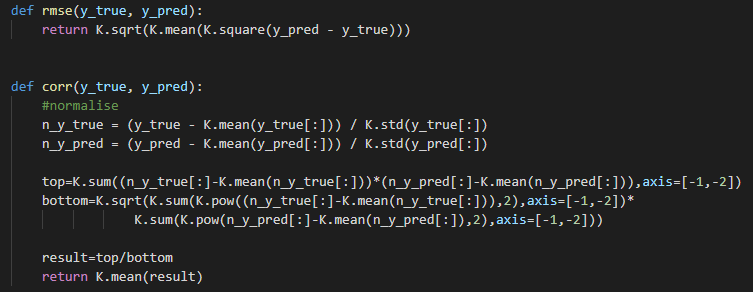
\includegraphics[angle=0, width=0.9\textwidth]{Figures/model_metrics.PNG}
  \caption{Model Custom Metrics}
  \label{fig:ModelCustomMetrics}
  \end{center}
\end{figure}


%%%%%%%%%%%%%%%%%%%%%%%%%%%%%%%%%%%%%%%%%%%%%%%%%%%%%%%
\section{Regularization}
A central role in developing a successful solution with Machine Learning is making sure that an algorithm will perform well not only on the training data, but also on previously unseen data. In many Machine Learning challenges it is common, that a well performing algorithm on the training data performs bad on previously unseen data. This behaviour is called 'Overfitting'. Strategies explicitly designed for decreasing decreasing Overfitting, even at the expense of increasing the training error, are known as regularization. \citep{Goodfellow:2016:DeepLearning}
\newline\newline
In order to prevent overfitting and generalize a model better, \citet{Chollet:2017:DeepLearningPython} highlights that the best solution is to get more training data. Provided that the model could be exposed to infinite data, it would never overfit. However, when it is not possible to expose the model to more data, \citet{Chollet:2017:DeepLearningPython} recommends utilizing regularization techniques, which will force the model to focus on the most prominent patterns. These techniques constrain the model in a way that it can only store a certain amount or certain type of information. According to \citet{Chollet:2017:DeepLearningPython}, the easiest way to prevent overfitting is to reduce the network's size or in other words to remove features. As a result, the number of trainable parameters in the model is reduced and thus, the model's capacity shrinks.

\subsubsection{Feature removal}
For the here proposed Machine Learning model it is indeed not possible to get more training data, as this would make an objective comparison with benchmark paper impossible. Thus, further regularization techniques have been applied. The first choice, was also to reduce the network's size. The pre-trained VGGFace network already provides a big stack of layers that cannot be removed without loosing valuable information. Therefore, the custom layers were reduced to a single Dense layer, which was proposed in a similar way by \citet{Pittaras:2017:FineTuningStrategiesComparison}.

\subsubsection{Dropout}
According to \citet{Chollet:2017:DeepLearningPython}, Dropout is one of the most effective and commonly used regularization techniques. When applied, noise is introduced during training by randomly setting a certain percentage of the layer's output values to zero. The Dropout applied in the proposed architecture was determined through extensive experimentation and gets applied before and after the single Dense layer with a rate of 0.7 and 0.6 respectively. The following figure shows an example with a dropout rate of 0.5.

\begin{figure}[H]
  \begin{center}
  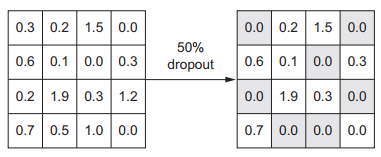
\includegraphics[angle=0, width=0.7\textwidth]{Figures/dropout.PNG}
  \caption{Dropout applied to an activation matrix at training time.\citep{Chollet:2017:DeepLearningPython}}
  \label{fig:Dropout}
  \end{center}
\end{figure}

\subsubsection{DataAugmentation}
Data Augmentation is another technique that is used to increase noise during training by randomly transforming existing training samples into slightly different looking images. As \citet{Chollet:2017:DeepLearningPython} argues, that Data Augmentation is exposing the model to more aspects of the data, as it will never see the exact same picture twice. As a result, the model will generalize better.
The Data Augmentation applied in the here proposed solution is augmenting the images randomly with the following parameters:

\begin{itemize}
    \item rotation range from 0 to 30 degrees
    \item width shift range from 0 to 25 percent of the total width
    \item height shift range from 0 to 25 percent of the total width
    \item horizontal flip
    \item brightness shift range from 50 to 150 percent
    \item zoom range from 0 to 30 percent
\end{itemize}


\subsubsection{Early Stopping}
Early Stopping is a callback that can be injected into the learning process of the Machine Learning model. Instead of running the training for a specified number of epochs, the Early Stopping callback can define a different criterium for the model to stop early. In the case of the here proposed solution, the Early Stopping callback monitors the validation loss metric and stops training 20 consecutive epochs after the last improvement on the validation loss was observed. The definition of this callback looks like this:

\begin{figure}[H]
  \begin{center}
  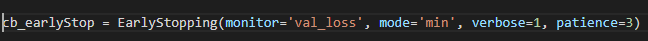
\includegraphics[angle=0, width=0.8\textwidth]{Figures/EarlyStopping.PNG}
  \caption{Early Stopping Callback}
  \label{fig:EarlyStopping}
  \end{center}
\end{figure}

The Early Stopping callback gets combined with a Model Checkpoint callback that keeps track of the best model during training and saves it to a predefined destination. The Model Checkpoint callback in the proposed solution monitors also the validation loss and saves the current weights of the model at the point of the validation loss being the lowest. The definition of this callback loss like this:

\begin{figure}[H]
  \begin{center}
  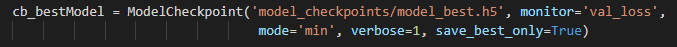
\includegraphics[angle=0, width=0.8\textwidth]{Figures/ModelCheckpoint.PNG}
  \caption{Model Checkpoint Callback}
  \label{fig:ModelCheckpoint}
  \end{center}
\end{figure}

To sum up, these two callbacks, the Early Stopping and the Model Checkpoint, keep track of the validation loss metric and interrupt training as soon as there is no improvement for 20 consecutive epochs. When this happens, it automatically backups the weights of the model at the point when the validation loss achieved the best, and lowest, result.

\subsubsection{Hyper-parameter optimization}
Another crucial impact for reducing the effects of overfitting can be contributed to the optimization of important hyper-parameters. Probably the two most impacting parameters are the learning rate and batch size.
\newline\newline
An analysis conducted by \citet{Yuanzhi:2019:RegularizationInitialLargeLearningRate} on Initial Learning Rates confirms that an initial large learning rate can have a regularization effect. Even though a small initial learning rate might allow for better performance initially, it will not be able to generalize as well as initial large learning rates. Therefore, the training in the approach proposed in this Master thesis makes use of an initial learning rate of 0.0001 for the first 3 epochs. Afterwards it gets lowered even down to 0.00001 \hl{further lowered?}.
\newline\newline
Next to the effects of the initial learning rate on improving generalization and thus reducing the effects of overfitting, \citet{Keskar:2016:LargeBatchTrainingGeneralization} support with experiments that choosing small-batch methods consistently generalize better than large-batch methods. Summing up, both the learning rate and batch size can offer a regularizing effect due to the noise they add during the training process.

\hl{L2 regularizer / kernel regularizer ???}
% # Applying kernel regularizer (which in the current status wasn't chosen)
% Reducing overfitting through applying regularization to pretrained neural networks
% https://sthalles.github.io/keras-regularizer/
